\newpage
\subsection{Konzept Grün}
\label{KonzeptGreen}
Konzept Grün besteht aus diesen Teillösungen: asfökjlsdföklsdfjsdöflsdjöklfsdöjklf
\newline

\subsubsection{Vereinzelung durch Wendelförderer}
\begin{wrapfigure}[13]{r}{7.5cm}
	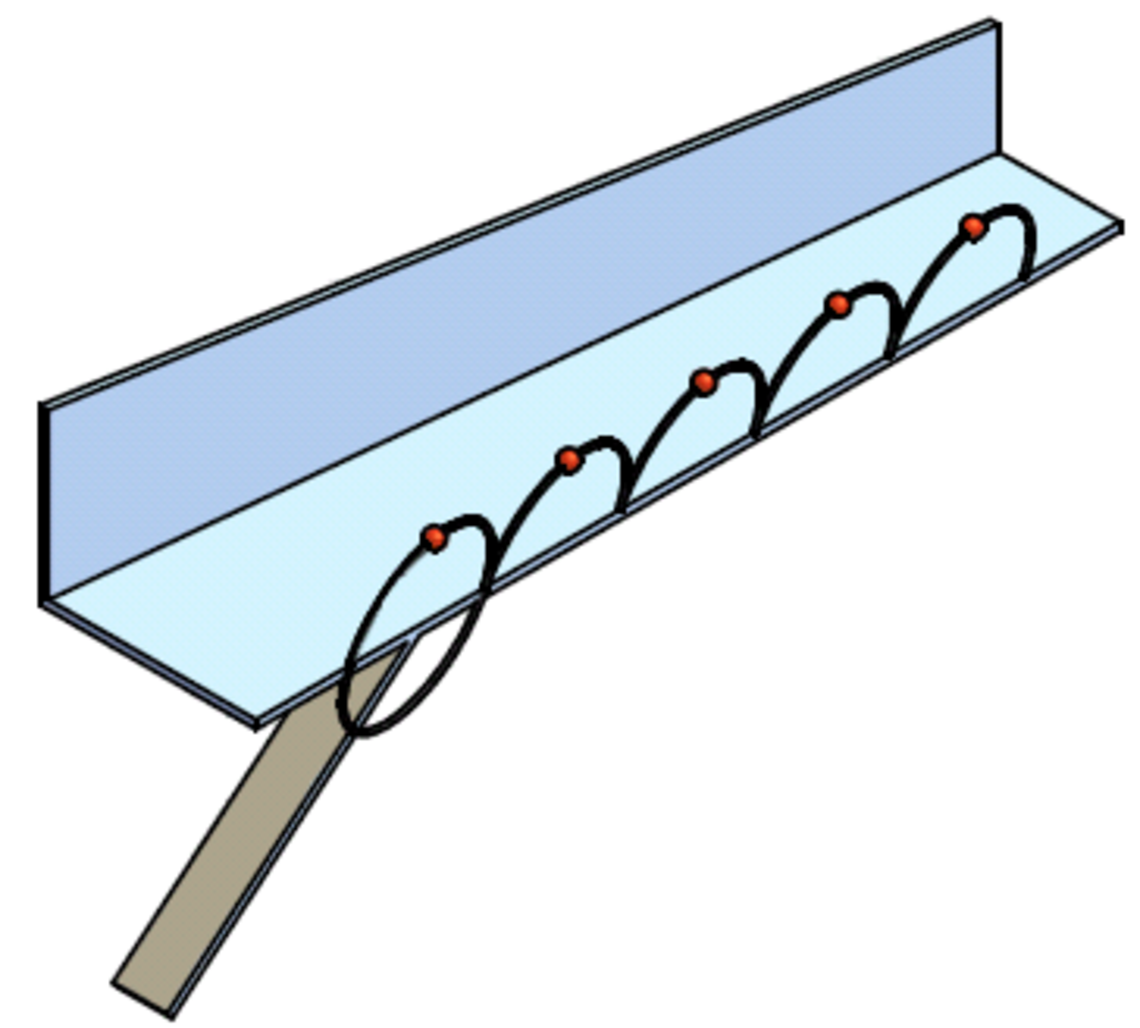
\includegraphics[scale=0.2]{Illustrationen/5-Konzept/foerderbewegung.png}
	\caption{Wurfbewegung erzeugt durch Vibration}
	\label{fig:foerderbewegung}
\end{wrapfigure}
Das Konzept Grün beinhaltet die Verzeinzelung sowie Förderung von NemaCaps mit einem Vibrationswendelförderer (siehe Abbildung \ref{fig:vereinzelung_green}). Vibration ist für die Vereinzelung sowie Förderung von Gütern mit einfacher Geometrie oft genutzte Technik. Dabei wird nach Webac GmbH (2017) mittels Schwingungsenergie (erzeugt durch eine Unwuchterregung mittels Vibrator) die zu bewegende Masse erregt und eine Hin- und Rückbewegung erzeugt. Dabei wird die Masse so angestossen, dass eine Kette von Wurfbewegungen entsteht und sich die Masse fortbewegt (siehe Abbildung \ref{fig:foerderbewegung}).

\begin{wrapfigure}[14]{r}{7.5cm}
	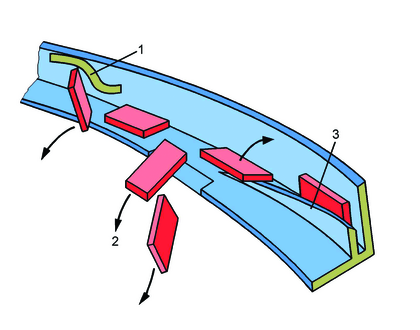
\includegraphics[scale=2.0]{Illustrationen/5-Konzept/schikane.png}
	\caption{Vereinzelung durch Schikanen}
	\label{fig:schikane}
\end{wrapfigure}


Die Vereinzelung wird mit Schikanen realisiert. Diese gewährleisten durch Abstimmung der Werkstückkontur, dass jeweils nur ein Werkstück die Schikane passiert und weiter gefördert wird (siehe Abbildung \ref{fig:schikane}). Überzählige werden zurück ins Haufwerk gelenkt (Handling online, 2006).
\newline
Der vorgesehene Wendelförderer basiert auf den erwähnten Techniken. In einer Spirale werden durch die Vibration die Werkstücke gefördert und sogleich vereinzelt. Speziell an dieser Anwendung ist, dass die NemaCaps in drei parallele Bahnen geteilt werden. Auch denkbar ist die Verwendung von drei einzelnen Wendelförderer.
\newline
\begin{figure}[H]
	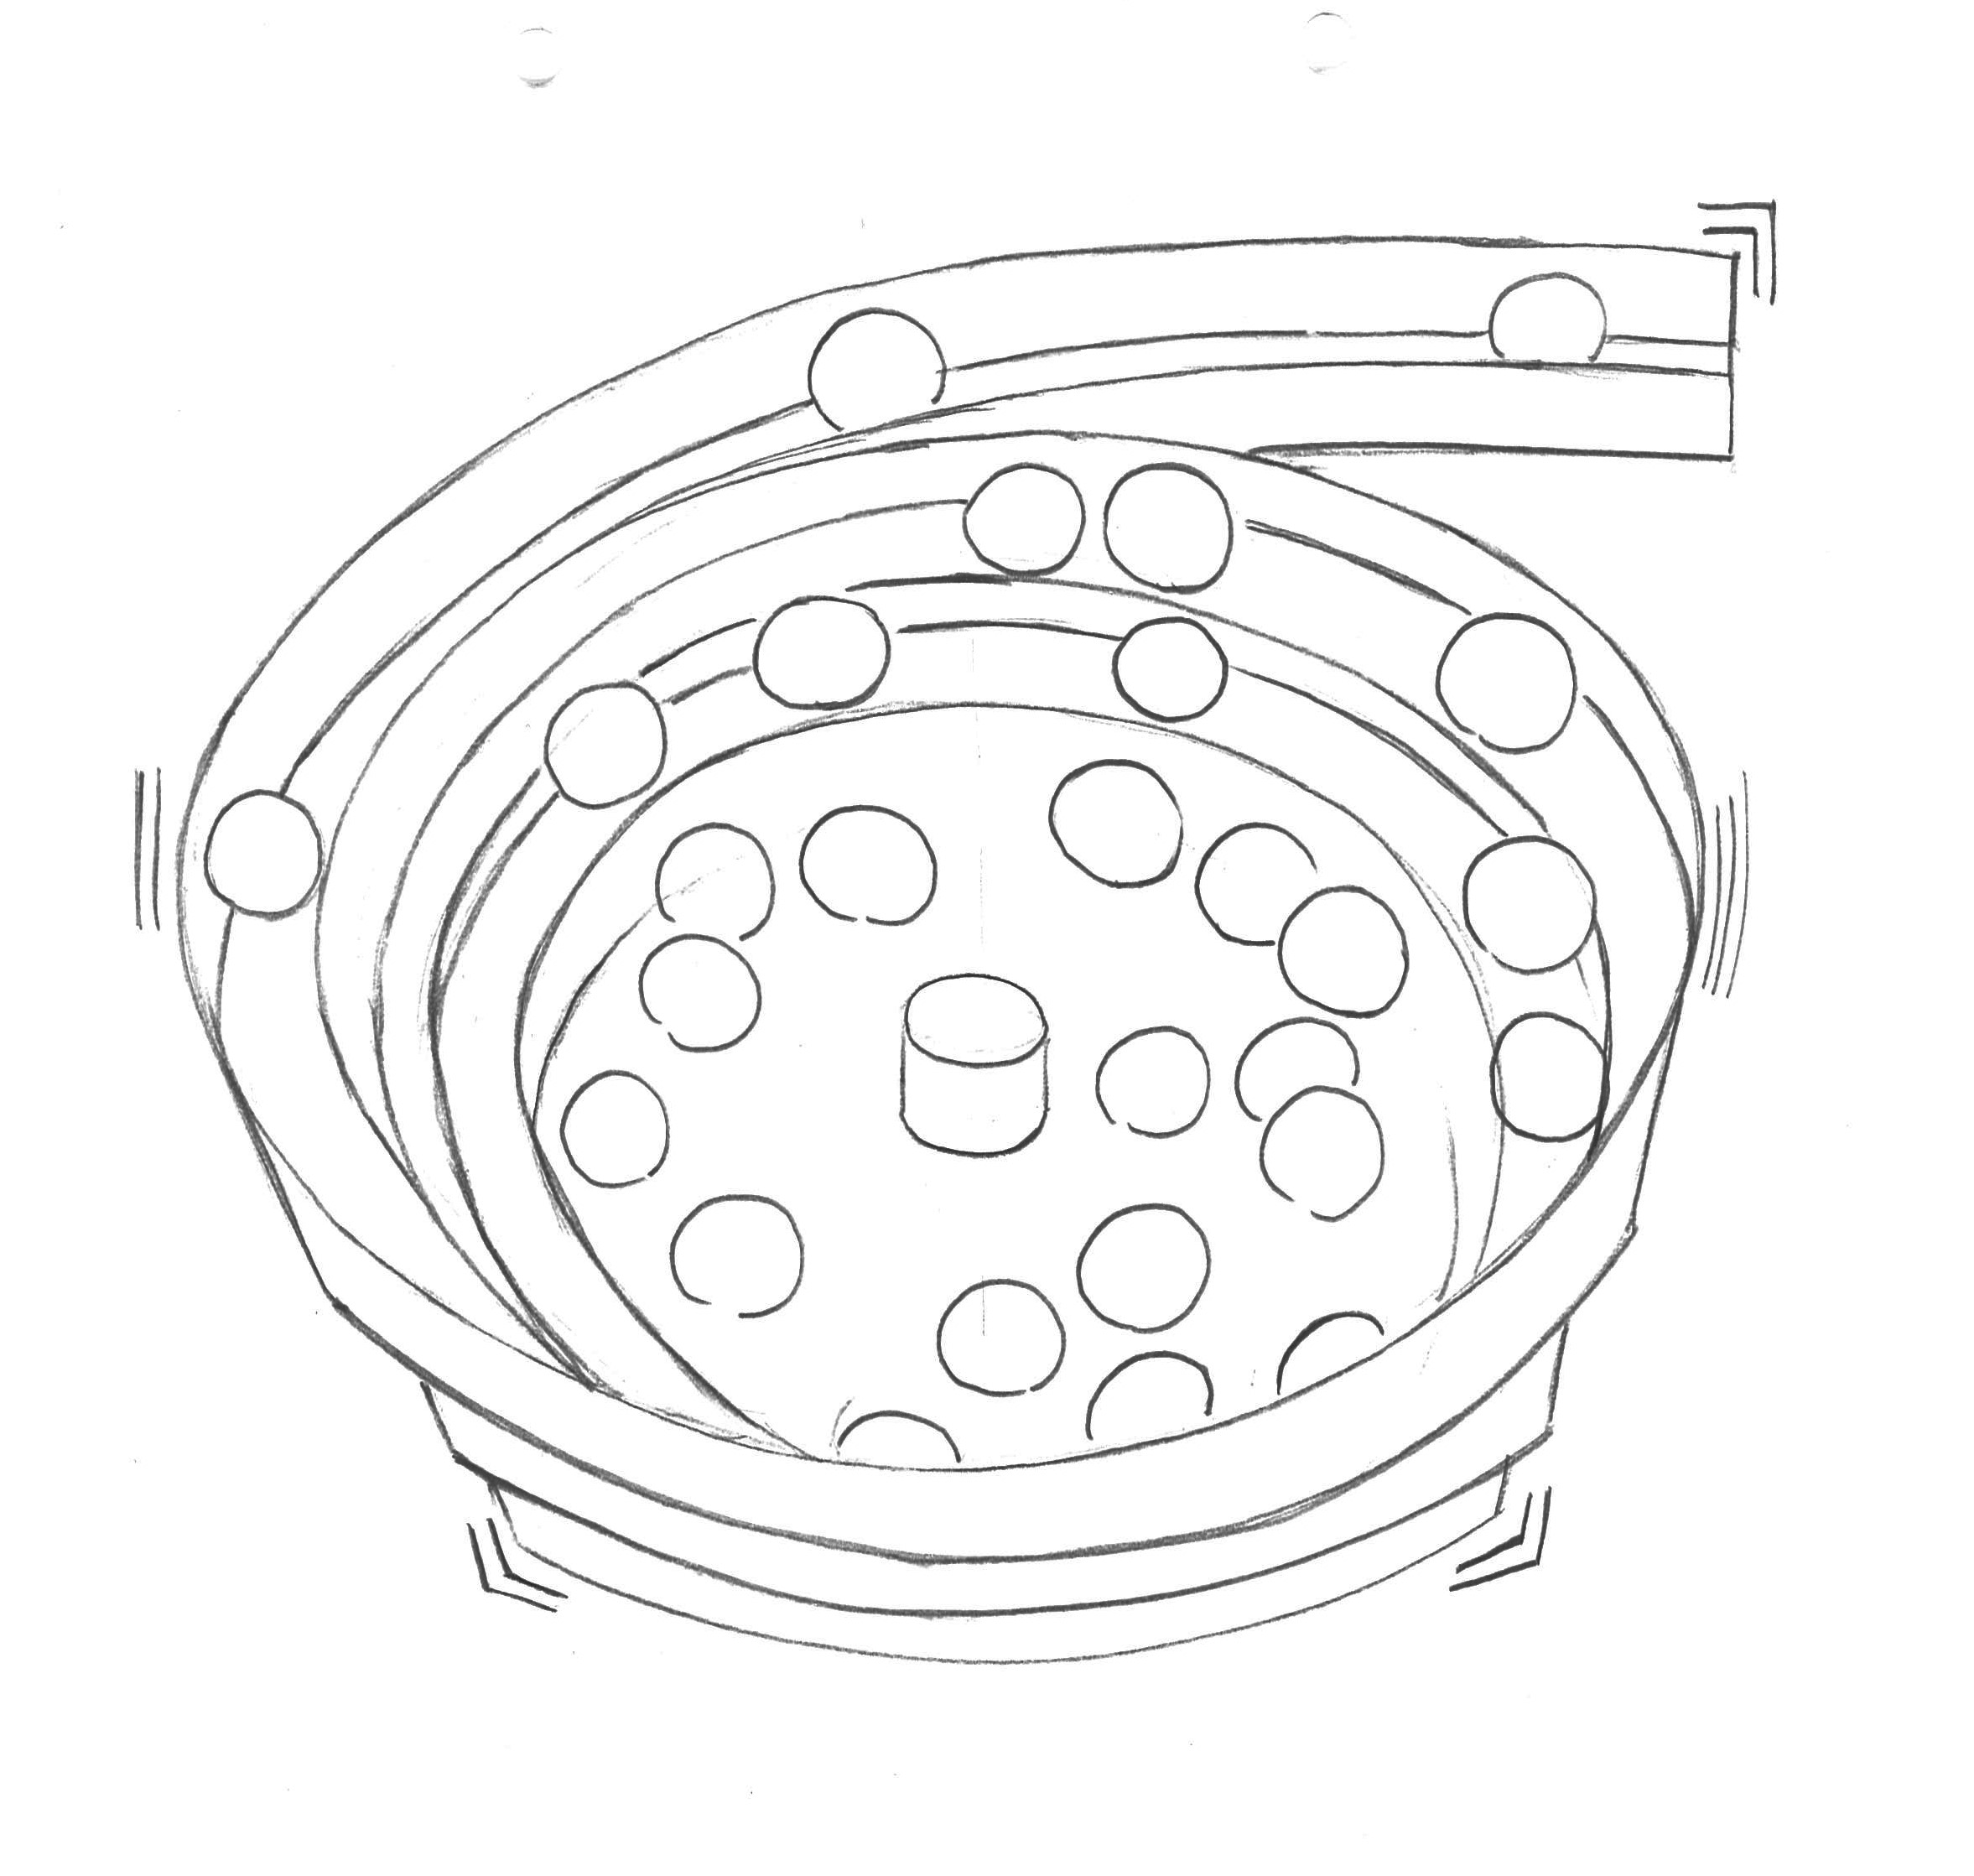
\includegraphics[scale=0.6]{Illustrationen/5-Konzept/green_wendelfoerderer.jpg}
	\caption{Konzeptskizze I Konzept Grün: Wendelförderer}
	\label{fig:vereinzelung_green}
\end{figure}

\textbf{Setzen mittels Pick-and-Place Bewegung}
\newline
Die NemaCaps kommen geordnet bei der Setzeinheit an. Dabei werden diese an einem mechanischen Anschlag gestoppt (Siehe Punkt 1 in Abbildung XY). Von dort werden die NemaCaps durch eine Setzeinheit gepackt und in den Töpfen platziert. Dabei ist die Setzeinheit als zweidimensionale Pick-and-Place Maschine aufgebaut. Diese zwei Dimensionen sind:
\begin{itemize}
	\item Translation in X-Richtung: Diese Bewegung dient zum horizontalen Transport von mechanischem Anschlag zum Topf.
	\item Translation in Z-Richtung: Um das NemaCap zu Packen sowie im Topf zu platzieren wird diese Bewegung ausgeführt.
\end{itemize}
Zur Übersicht dient Abbildung \ref{fig:transport_green_pers}. 
\begin{figure}[H]
	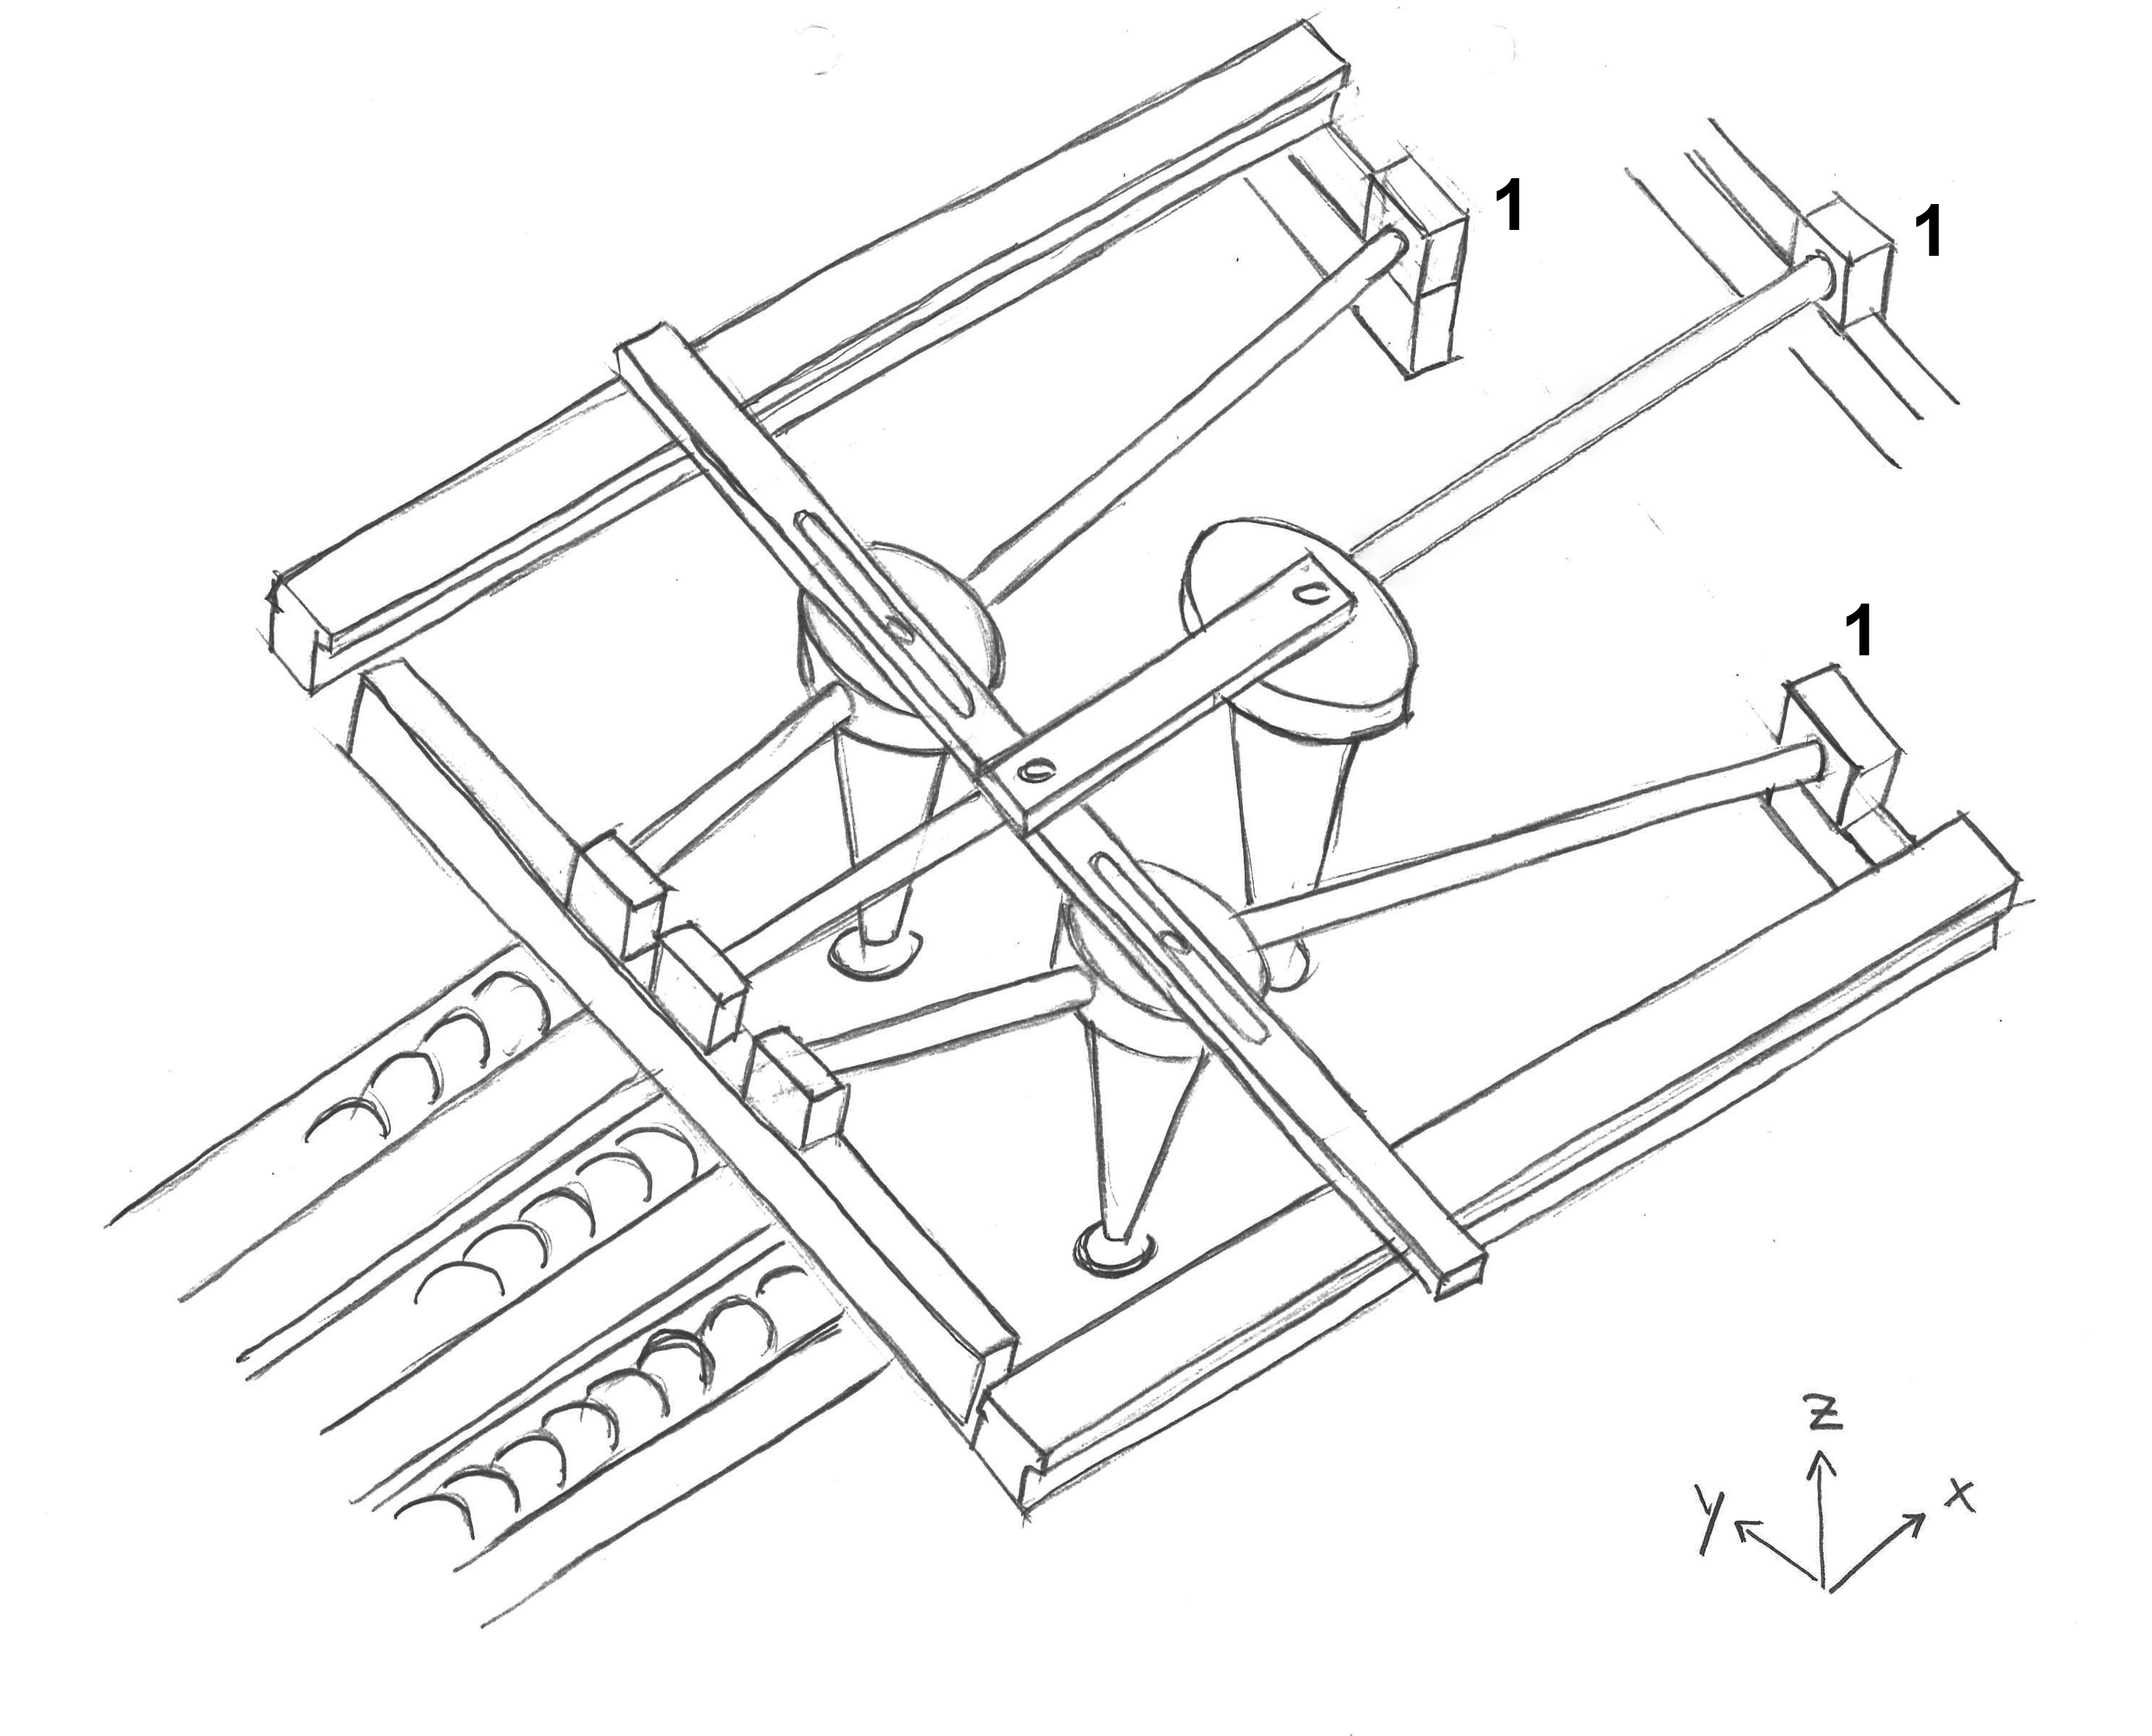
\includegraphics[scale=0.6]{Illustrationen/5-Konzept/green_2Dmachine_pervsp.jpg}
	\caption{Konzeptskizze II Konzept Grün: Perspektivische Ansicht der Pick-and-Place Bewegung}
	\label{fig:transport_green_pers}
\end{figure}

Der Prozess der Setzeinheit gestaltet sich folgendermassen:
\begin{itemize}
	\item \textbf{A - NemaCap packen:} Sobald der bewegte Teil der Seitzeinheit sich über dem NemaCap befindet, packen drei Dorne je ein NemaCap (Detail A in Abbildung XY). Für das Packen sind folgende Techniken möglich:
	\begin{itemize}
		\item Mittels Zange wird das NemaCap seitlich gefasst.
		\item Durch einen spitzen Dorn wird das NemaCap aufgespiesst (Gemäss Pflichtenheft zulässig).
		\item Durch einen stumpfen Dorn mit hoher Adhäsion (zum Beispiel Kleber) wird das NemaCap angeheftet.
		\item Mittels Unterdruck wird das NemaCap an eingem Dorn angesaugt.
	\end{itemize} 
	\item \textbf{B - NemaCap transportieren:} Das NemaCap wird durch die Bewegung in X-Richtung über die Einsatzlokalität transportiert. Dabei werden die einzelnen Dorne durch Laufschienen geleitet und so auf den entprechenden Topfradius gelenkt. Die einzelnen Dorne sind miteinander verbunden, sodass diese lineare Bewegung nur ein Aktor erfordert.
	\item \textbf{A - NemaCap setzen:} 
	Über der Einsetzlokalität angekommen, bewegt sich der Dorn in Z-Richtung nach unten und stösst das NemaCap in die Erde. Dabei wird eine Beschädigung des NemaCaps bewusst in Kauf genommen, da dies gemäss Pflichtenheft zulässig ist. Wichtig ist, dass beim Zurückfahren des Dorns sich das NemaCap vom Dorn löst.
\end{itemize}
Die Konfiguration des Setzmechanismus ist durch die Verstellung der Laufschienen möglich. Dabei sind die Laufschienen am oberen Ende (über dem Topf) in Y-Richtung verstellbar. So können die verschiedenen Topfgrössen gehandhabt werden.

\begin{figure}[H]
	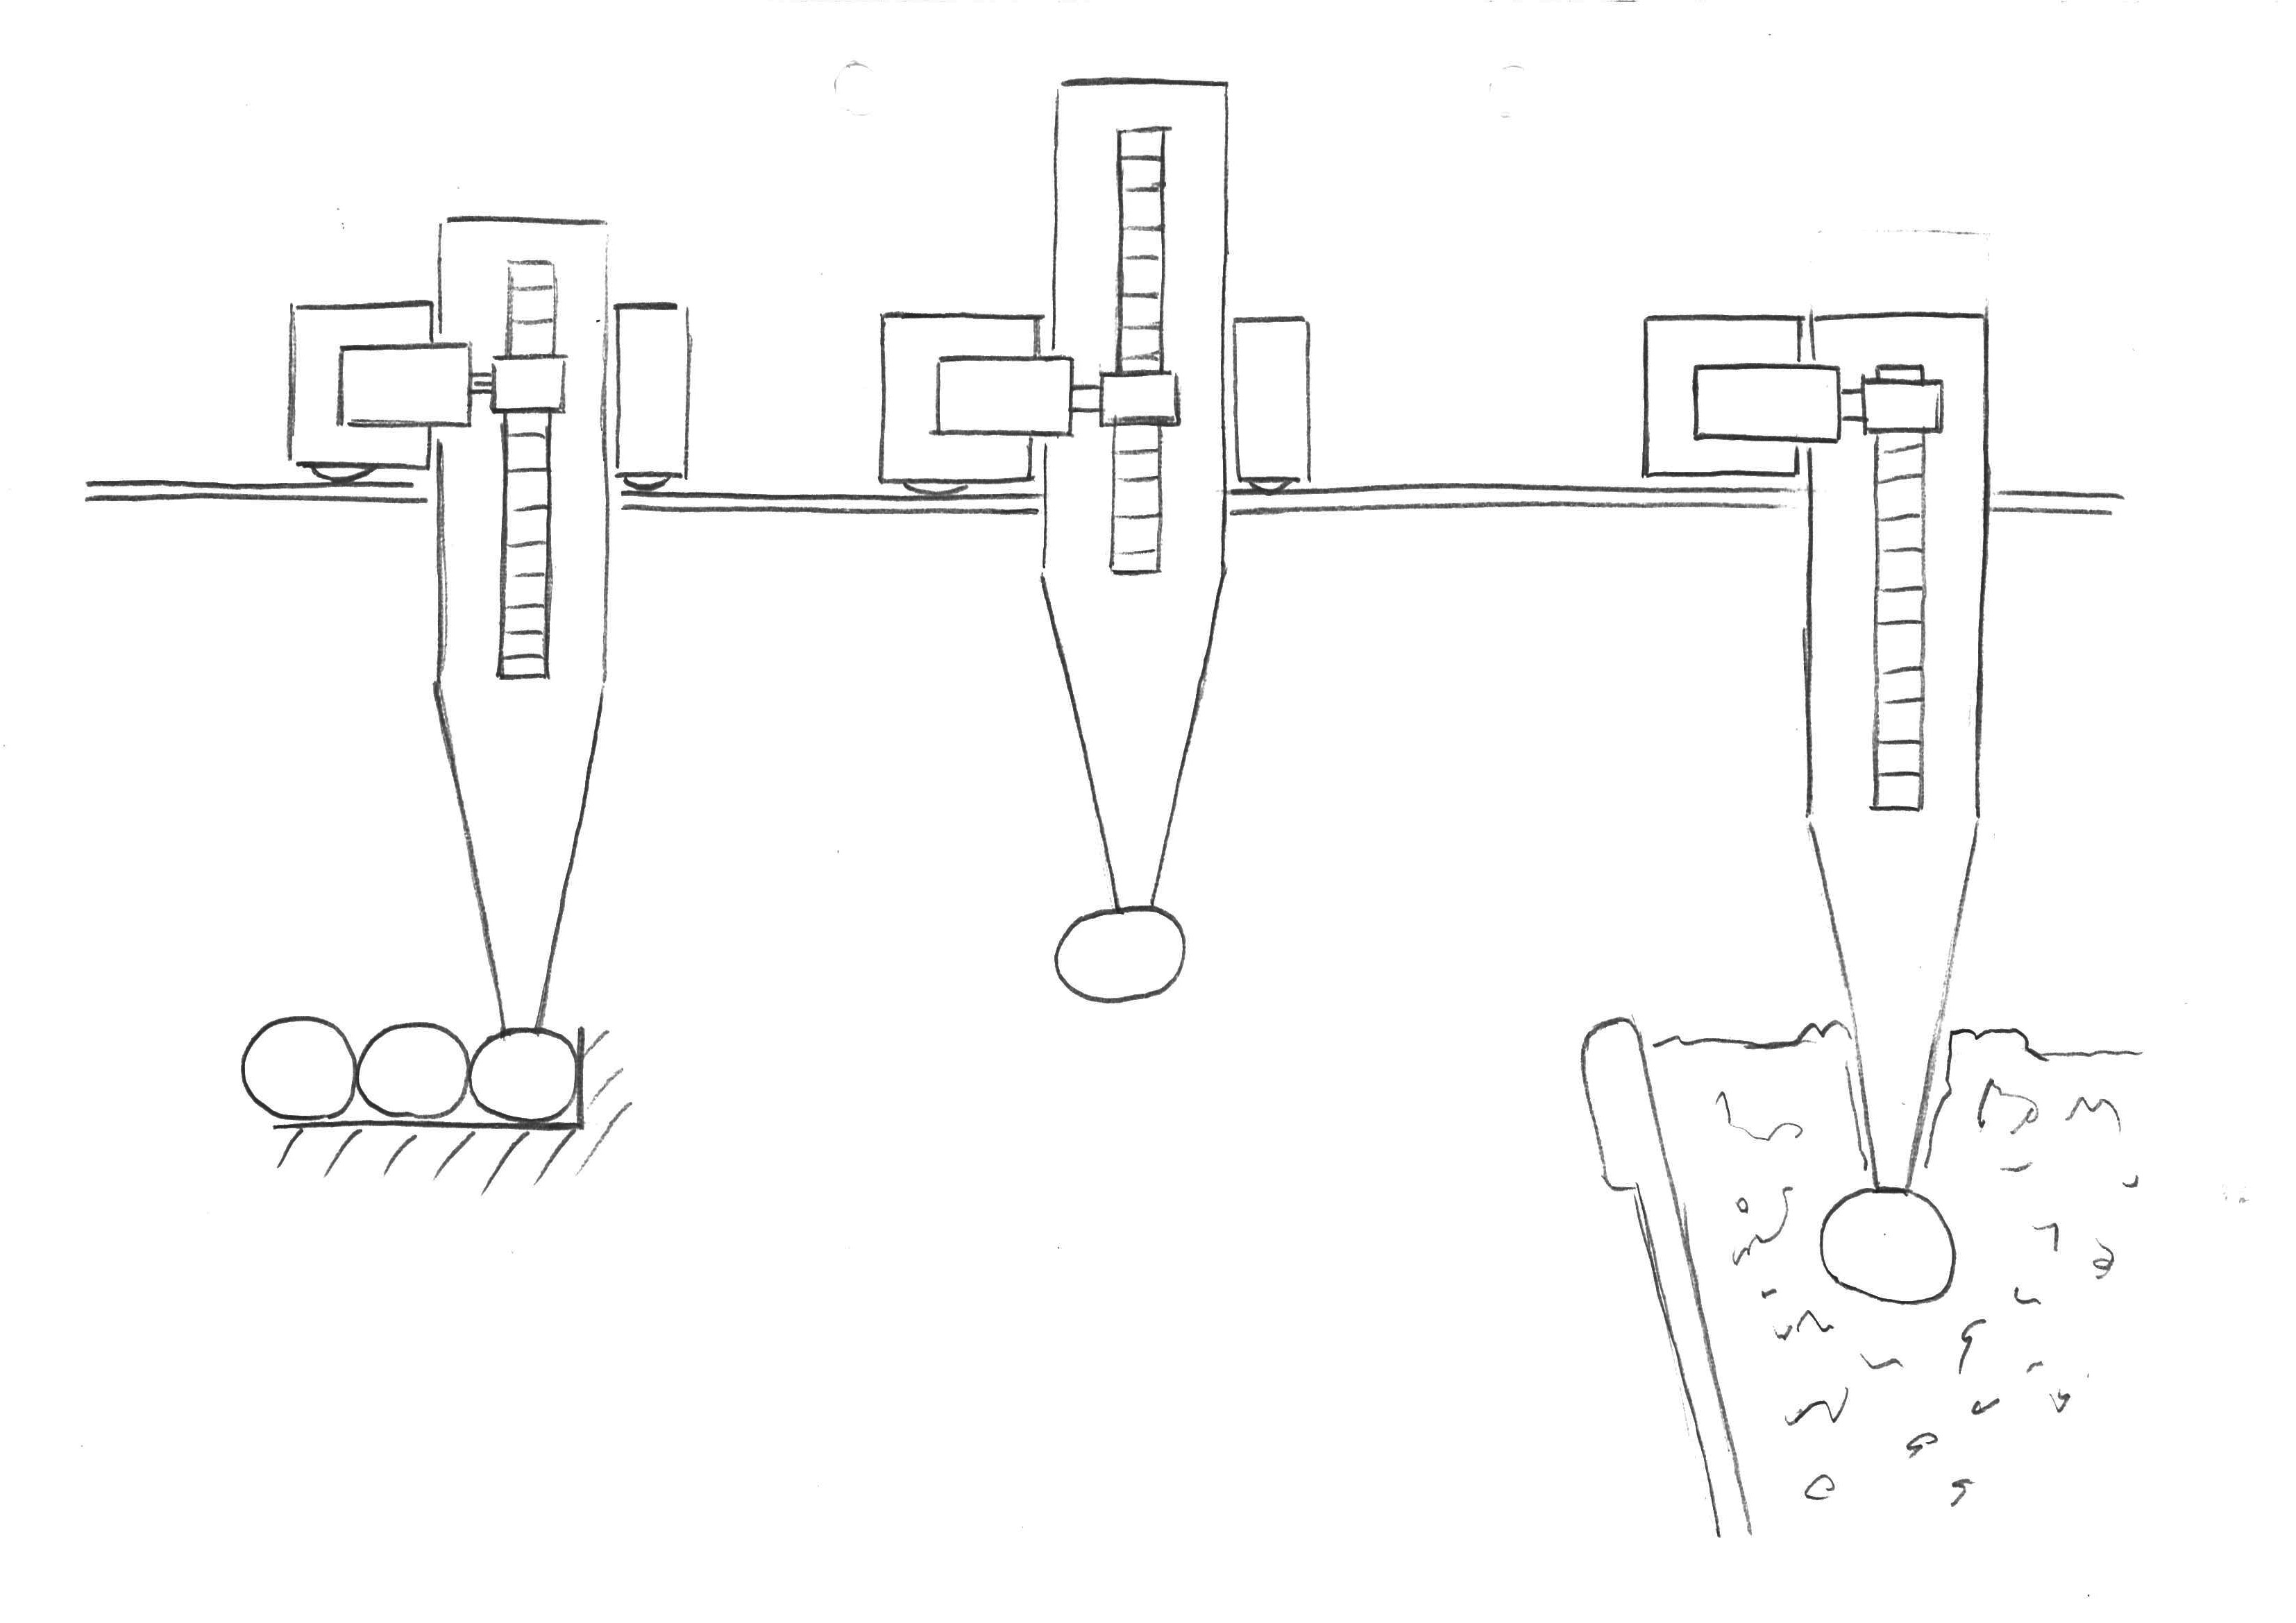
\includegraphics[scale=0.6]{Illustrationen/5-Konzept/green_2Dmachine_seite.jpg}
	\caption{Konzeptskizze III Konzept Grün: Seitenansicht der Pick-and-Place Bewegung}
	\label{fig:transport_green_side}
\end{figure}